\documentclass[../TDT3.tex]{subfiles}%

\begin{document}
\section[s]"3"{Chauffage d'une chambre}

\enonce{%
	On étudie le chauffage d'une chambre au dernier étage de l'internat en hiver.
	On installe un radiateur électrique d'appoint fournissant une puissance de
	chauffe $\Pc_c$. Le volume de la chambre est $V = \SI{36}{m^3}$, et est rempli
	d'air de capacité thermique molaire $C_{V,m} = \frac{5}{2}R$. On la suppose
	vide de meubles.
	\smallbreak
	Les échanges thermiques se font \textit{via} par deux surfaces~: le mur et les
	vitres en contact avec l'extérieur et le toit, de surfaces égales $S =
		\SI{12}{m^2}$. Les autres surfaces sont supposées à l'équilibre thermique du
	fait des chambres voisines et en-dessous. On note $T\ind{int}(t)$ la
	température intérieure, et $T\ind{ext} = \SI{10}{\degreeCelsius}$ la
	température extérieure, supposée constante.
	\smallbreak
	Les fuites thermiques à la date $t$ à travers le mur sont données par la
	puissance $\Pc\ind{mur} = g\ind{mur}S (T\ind{int}(t) - T\ind{ext})$, et celles
	à travers le toit par $\Pc\ind{toit} = g\ind{toit}S (T\ind{int}(t) -
		T\ind{ext})$.
	\smallbreak
	On souhaite maintenir la température à une température de confort $T_c =
		\SI{19}{\degreeCelsius}$. La pression de l'air intérieur est $P_0 =
		\SI{1.0}{bar}$ à cette température.
	\begin{tcn}(data)<lfnt>{Données}
		$g\ind{mur} = \SI{2.90}{W.m^{-2}.K^{-1}}$ et $g\ind{toit} =
			\SI{0.50}{W.m^{-2}.K^{-1}}$, $R = \SI{8.314}{J.K^{-1}.mol^{-1}}$.
	\end{tcn}
}%
\QR{%
	Faire un schéma représentant la pièce, le radiateur et l'extérieur, en faisant
	apparaître les transferts thermiques entrant en rouge et les transferts
	thermiques sortant en bleu.
}{%
	\sswitch{
		\hfill
		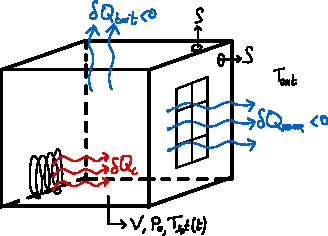
\includegraphics[width=.4\linewidth, valign=t]{E7_chambre}
		\hspace*{\fill}
	}{
		\vspace{-30pt}
		\begin{center}
			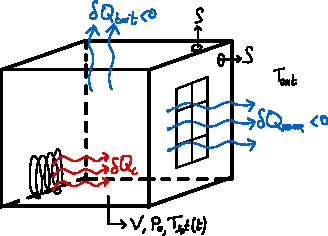
\includegraphics[width=.4\linewidth]{E7_chambre}
		\end{center}
	}
}%
\QR{%
	Calculer le nombre de moles d'air présentes dans la chambre dans les
	conditions $(T_c,P_0)$. En déduire la capacité thermique $C_V$ de l'air
	contenu dans la chambre. Faire l'application numérique.
}{%
	\begin{gather*}
		P_0V = nRT_c
		\Lra
		\boxed{n = \frac{P_0V}{RT_c}}
		\qav
		\left\{
		\begin{array}{rcl}
			P_0 & = & \SI{1e5}{Pa}
			\\
			V   & = & \SI{36}{m^3}
			\\
			R   & = & \SI{8.314}{J.K^{-1}.mol^{-1}}
			\\
			T_c & = & \SI{292}{K}
		\end{array}
		\right.\\
		\AN
		\xul{
			n = \SI{1.5e3}{mol}
		}
		\\\beforetext{Par définition,}
		C_{V,m} = \frac{C_V}{n}
		\Lra
		\boxed{C_V = n C_{V,m}}
		\Ra
		\xul{C_V = \SI{31}{kJ.K^{-1}}}
	\end{gather*}
}%
\QR{%
	Quelle est la puissance $\Pc_c$ fournie par le radiateur pour maintenir une
	telle température de confort dans les conditions mentionnées ci-dessus~?
}{%
	Le volume de la chambre étant fixé, il n'y a pas de $W_p$. Si la température
	est constante, c'est que le radiateur \textbf{compense les pertes}, et on a
	que $\dd{U} = C_V \dd{T} = 0$. Ainsi, avec le premier principe,
	\begin{DispWithArrows*}
		\dd{U} &= \delta{Q_c} + \delta{Q\ind{toit}} + \delta{Q\ind{mur}}
		\Arrow{$\delta{Q}\ind{toit} < 0$\\$\delta{Q}\ind{mur} < 0$}
		\\\Lra
		0 &= \Pc_c \dd{t} - \Pc\ind{toit} \dd{t} - \Pc\ind{mut}\dd{t}
		\\\Lra
		\Pc_c = \Pc\ind{toit} + \Pc\ind{mur}
		\\\Lra
		\Aboxed{\Pc_c = (g\ind{toit} + g\ind{mur})S (T_c-T\ind{ext})}
		\qav
		\left\{
		\begin{array}{rcl}
			g\ind{toit} & = & \SI{0.50}{W.m^{-2}.K^{-1}}
			\\
			g\ind{mur}  & = & \SI{2.90}{W.m^{-2}.K^{-1}}
			\\
			S           & = & \SI{12}{m^2}
			\\
			T_c         & = & \SI{292}{K}
			\\
			T\ind{ext}  & = & \SI{283}{K}
		\end{array}
		\right.\\
		\makebox[0pt][l]{$\phantom{\AN}\xul{\phantom{\Pc_c = \SI{3.7e2}{W}}}$}
		\AN
		\Pc_c &= \SI{3.7e2}{W}
	\end{DispWithArrows*}
	\begin{tcb}(rema){Remarque}
		Les expressions de $\Pc\ind{mur}$ et $\Pc\ind{toit}$ montrent qu'il n'y a
		logiquement pas de fuite si $T\ind{int} = T\ind{ext}$, et que $P\ind{mur}$
		et $P\ind{toit} \propto S$ puisque plus la surface est grande plus il y a de
		fuite. Cela se retrouve dans l'unité donnée.
	\end{tcb}
}%
\enonce{%
	On doit partir pour une khôlle et dîner, et on se demande s'il vaut mieux
	couper le chauffage ou le maintenir. On suppose alors qu'on arrête le
	chauffage à $t=0$, et qu'on revient \SI{3}{h} plus tard au temps $t_1$.
}%
\QR{%
	En supposant qu'il n'y a pas de circulation d'air, appliquer le premier
	principe sous forme différentielle à l'air de la chambre et déterminer
	l'équation différentielle vérifier par $T\ind{int}(t)$ pour $t \in [0,t_1]$.
	On introduira un temps caractéristique $\tau$ que l'on calculera.
}{%
	On a encore $\dd{V} = 0 \Ra \delta{W}_p = 0$, et il n'y a que les pertes
	thermiques puisqu'on a coupé le chauffage. Ainsi,
	\begin{align*}
		\dd{U}                                       & = \sum_i \dd{Q}_i
		\\\Lra
		C_V \dd{T}\ind{int}                          & = -(\Pc\ind{toit} + \Pc\ind{mur})\dd{t}
		\\\Lra
		C_V \dv{T\ind{int}}{t}                       & =
		-(g\ind{toit} + g\ind{mur})S (T\ind{int} - T\ind{ext})
		\\\Lra
		\dv{T\ind{int}}{t} + \frac{(g\ind{toit} + g\ind{mur})S}{C_V}T\ind{int}
		                                             & =
		\frac{(g\ind{toit} + g\ind{mur})S}{C_V} T\ind{ext}
		\\\Lra
		\Aboxed{
		\dv{T\ind{int}}{t} + \frac{T\ind{int}}{\tau} & = \frac{T\ind{ext}}{\tau}
		}
		\qav
		\boxed{\tau = \frac{C_V}{(g\ind{toit} + g\ind{mur})S}}
		\Ra
		\xul{\tau = \SI{7.6e2}{s} \approx \SI{13}{min}}
	\end{align*}
}%
\QR{%
	Résoudre cette équation différentielle, puis tracer cette évolution au cours
	du temps, et déterminer la température $T\ind{int,f}$ lors du retour dans la
	chambre.
}{%
	\noindent
	\begin{minipage}[t]{.70\linewidth}
		\begin{align*}
			\beforetext{Solution particulière~:}
			T\ind{int,p}  & = T\ind{ext}
			\\\beforetext{Solution homogène~:}
			T\ind{int,h}  & = K\exr^{-t/\tau}
			\\\beforetext{Solution totale~:}
			T\ind{int}(t) & =
			T\ind{int,p} + T\ind{int,h} = T\ind{ext} + K\exr^{-t/\tau}
			\\\beforetext{Condition initiale~:}
			T\ind{int}(0) & = T_c
			\\\Lra
			T_c           & = T\ind{ext} + K
			\\\Lra
			K             & = T_c - T\ind{ext}
			\\\beforetext{Solution finale~:}
			\Lra
			\Aboxed{
			T\ind{int}(t) & = T\ind{ext} + (T_c - T\ind{ext})\exr^{-t/\tau}
			}
		\end{align*}
	\end{minipage}
	\hfill
	\begin{minipage}[t]{.35\linewidth}
		\vspace{0pt}
		\hspace*{-2cm}
		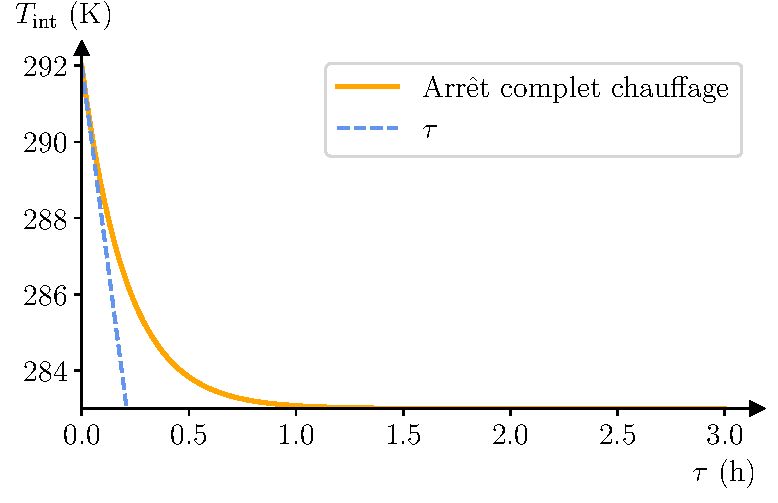
\includegraphics[width=1.2\linewidth]{E7_eqdiff}
	\end{minipage}
	On a une exponentielle décroissante avec $\tau \approx \SI{13}{min}$. Or, au
	bout de $t \approx 5\tau$ on sait que la solution particulière est atteinte,
	donc au bout de $t \approx \SI{1}{h}$ la chambre a complètement refroidi.
	Quand on revient après \SI{3}{h}, il fait donc \SI{10}{\degreeCelsius} dans la
	chambre.
}%
\enonce{%
	On souhaite retrouver la température de confort $T_c$. Pour y revenir
	rapidement, on pousse la puissance de chauffe à son maximum,
	$\Pc_{c,\rm max} = \SI{2.0}{kW}$.
}%

\QR{%
	Écrire la nouvelle équation différentielle
	satisfaite par $T\ind{int}(t)$. Résoudre cette équation en prenant $t_1$ comme
	origine du temps (on considère $t_1 = 0$) et $T\ind{int,f}$ comme condition
	initiale, et exprimer la solution en fonction de $T\ind{ext}$, $T_c$,
	$\Pc_{c,\rm max}$, $\Pc_c$ et $\tau$.
}{%
	On rallume le chauffage, d'où
	\begin{align*}
		\dd{U}
		              & =
		\delta{Q}_{c,\rm max} + \sum_i \delta{Q}_i
		\\\Lra
		\dv{T\ind{int}}{t} + \frac{T\ind{int}}{\tau}
		              & =
		\frac{T\ind{ext}}{\tau} + \frac{\Pc_{c,\rm max}}{C_V}
		\intertext{Pour résoudre, on prend $t = t_1$ comme origine des temps, donc
			on écrira la solution initiale $T\ind{int}(0) = T\ind{ext}$ au lieu de
			$T\ind{int}(t_1) = T\ind{ext}$.}
		\beforetext{Solution particulière~:}
		T\ind{int,p}  & =
		T\ind{ext} + \frac{\tau}{C_V}\Pc_{c,\rm max} =
		T\ind{ext} + \frac{\Pc_{c,\rm max}}{(g\ind{toit}+g\ind{mur})S} =
		T\ind{ext} + \frac{\Pc_{c,\rm max}}{\Pc_c}(T_c-T\ind{ext})
		\\\beforetext{Solution homogène~:}
		T\ind{int,h}  & = K'\exr^{-t/\tau}
		\\\beforetext{Solution totale~:}
		T\ind{int}(t) & = T\ind{int,p} + T\ind{int,h} =
		T\ind{ext} +
		\frac{\Pc_{c,\rm max}}{\Pc_c}(T_c-T\ind{ext}) + K'\exr^{-t/\tau}
		\\\beforetext{Condition initiale~:}
		T\ind{int}(0) & = T\ind{ext}
		\\\Lra
		\cancel{T\ind{ext}}
		              & =
		\cancel{T\ind{ext}} +
		\frac{\Pc_{c,\rm max}}{\Pc_c}(T_c-T\ind{ext}) + K'
		\\\Lra
		K'            & = -\frac{\Pc_{c,\rm max}}{\Pc_c}(T_c-T\ind{ext})
		\\\beforetext{Solution finale~:}
		\Lra
		\Aboxed{
		T\ind{int}(t) & =
			T\ind{ext} +
			\frac{\Pc_{c,\rm max}}{\Pc_c}(T_c-T\ind{ext})(1-\exr^{-t/\tau})
		}
	\end{align*}
}%
\QR{%
	Tracer la solution obtenue, puis calculer la durée nécessaire pour
	retrouver la température de confort $T_c$. On appelle cet instant $t_2$.
}{%
	On trouve bien une exponentielle croissante. On trouve alors $t_2$ avec~:
	\smallbreak
	\noindent
	\begin{minipage}[c]{.60\linewidth}
		\begin{align*}
			T\ind{int}(t_2)
			    & =
			T_c
			\\\Lra
			T\ind{ext} +
			\frac{\Pc_{c,\rm max}}{\Pc_c}(T_c-T\ind{ext})(1-\exr^{-t_2/\tau})
			    & =
			T_c
			\\\Lra
			\frac{\Pc_{c,\rm max}}{\Pc_c} \cancel{(T_c - T\ind{ext})} (1-\exr^{-t_2/\tau})
			    & =
			\cancel{(T_c - T\ind{ext})}
			\\\Lra
			1 - \exr^{-t_2/\tau}
			    & =
			\frac{\Pc_c}{\Pc_{c,max}}
			\\\Lra
			\exr^{-t_2/\tau}
			    & =
			1 - \frac{\Pc_c}{\Pc_{c,\rm max}}
			\\\Lra
			-\frac{t_2}{\tau}
			    & =
			\ln (\frac{\Pc_{c,max} - \Pc_c}{\Pc_{c,max}})
			\\\Lra
			\Aboxed{
			t_2 & = \tau \ln (\frac{\Pc_{c,max}}{\Pc_{c,\rm max} -
					\Pc_c})
			}
			\\\makebox[0pt][l]{$\phantom{\AN}\xul{\phantom{t_2 = \SI{2.6}{min}}}$}
			\AN
			t_2 & = \SI{1.5e2}{s} = \SI{2.6}{min}
		\end{align*}
	\end{minipage}
	\hfill
	\begin{minipage}[c]{.40\linewidth}
		% \vspace{2.5cm}
		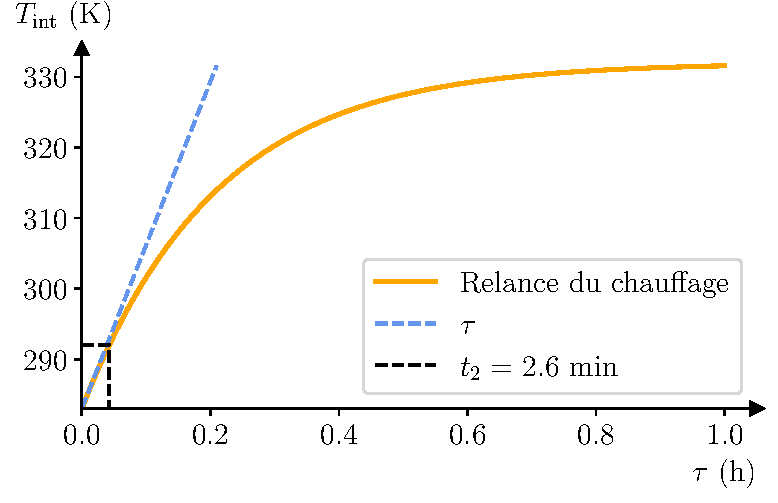
\includegraphics[width=\linewidth]{E7_eqdiff_rechauffe}
	\end{minipage}
}%

\QR{%
	Déterminer alors la différence d'énergie entre les deux situations~:
	\begin{itemize}
		\item On garde le chauffage à la puissance $\Pc_c$ de $t = 0$ à $t_2$~;
		\item On a éteint le chauffage de $t=0$ à $t_1$, mais on le rallume de $t_1$
		      à $t_2$ avec $\Pc_{c,\rm max}$.
	\end{itemize}
	On suppose que l'énergie électrique est parfaitement convertie en chaleur.
	Sachant que pour l'électricité on a $\SI{1}{kWh} \approx
		\SI{0.27}{\text{\euro}}$ avec l'augmentation de février 2024, déterminer
	l'écart financier entre ces deux méthodes. Commenter.
}{%
	\vspace{-15pt}
	\begin{itemize}
		\item[b]{On garde le chauffage}~: pendant $\Delta{t}_{02} \approx \SI{3}{h}
			= \SI{1.1e4}{s}$, on chauffe à la puissance $\Pc_c = \SI{3.7e2}{W}$, soit
		\begin{gather*}
			\boxed{Q\ind{garde} = \Pc_c\Delta{t}_{02}}
			\Ra
			\xul{Q\ind{garde} = \SI{4.0}{MJ}}
			\Lra
			\xul{Q\ind{garde,\euro} = \SI{0.30}{\text{\euro}}}
		\end{gather*}
		\item[b]{On éteint puis on rallume au maximum}~: on chauffe donc à
		$\Pc_{c,\rm max} = \SI{2.0}{kW}$ pendant $\Delta{t}_{12} = \SI{1.5e2}{s}$,
		soit
		\begin{gather*}
			\boxed{Q\ind{rechauffe} = \Pc_{c,\rm max}\Delta{t}_{12}}
			\Ra
			\xul{Q\ind{rechauffe} = \SI{3.1e-1}{MJ}}
			\Lra
			\xul{Q\ind{rechauffe,\euro} = \SI{0.023}{\text{\euro}}}
		\end{gather*}
	\end{itemize}
	Ainsi, pour une telle durée d'attente, il vaut mieux couper le chauffage~!
}%
\enonce{%
	On cherche maintenant à savoir s'il existe une durée $t_1$ telle que les deux
	méthodes soient similaires.
}%
\QR{%
	Reprendre la résolution de la seconde équation différentielle (réchauffage à
	$\Pc_{c,\rm max}$), avec pour condition initiale $T\ind{int}(t_1)$ la solution
	de la première équation différentielle (arrêt du chauffage)~: \textbf{on ne
		considère plus $t_1 = 0$ et $T\ind{int,f}$ comme conditions initiales}.
}{%
	\vspace{-15pt}
	\begin{align*}
		\beforetext{Solution particulière~:}
		T\ind{int,p}    & =
		T\ind{ext} + \frac{\Pc_{c,\rm max}}{\Pc_c}(T_c-T\ind{ext})
		\\\beforetext{Solution homogène~:}
		T\ind{int,h}    & = K''\exr^{-t/\tau}
		\\\beforetext{Solution totale~:}
		T\ind{int}(t)   & = T\ind{int,p} + T\ind{int,h} =
		T\ind{ext} +
		\frac{\Pc_{c,\rm max}}{\Pc_c}(T_c-T\ind{ext}) + K''\exr^{-t/\tau}
		\\\beforetext{Condition initiale~:}
		T\ind{int}(t_1) & = T\ind{ext} + (T_c - T\ind{ext})\exr^{-t_1/\tau}
		\\\Lra
		\cancel{T\ind{ext}} +
		\frac{\Pc_{c,\rm max}}{\Pc_c}(T_c-T\ind{ext}) +
		K''\exr^{-t_1/\tau}
		                & =
		\cancel{T\ind{ext}} +
		(T_c-T\ind{ext})\exr^{-t_1/\tau}
		\\\Lra
		K''\exr^{-t_1/\tau}
		                & =
		(T_c-T\ind{ext})\left[\exr^{-t_1/\tau} - \frac{\Pc_{c,\rm
					max}}{\Pc_c}\right]
		\\\Lra
		K''
		                & =
		(T_c - T\ind{ext}) \left[1 - \frac{\Pc_{c,\rm
					max}}{\Pc_c}\exr^{t_1/\tau}\right]
		\\\beforetext{Solution finale~:}
		\Lra
		\Aboxed{
		T\ind{int}(t)   & =
			T\ind{ext} +
			(T_c - T\ind{ext})
			\pac{\frac{\Pc_{c,\rm max}}{\Pc_c} +
				\exr^{-t/\tau}\pa{1 - \frac{\Pc_{c,\rm max}}{\Pc_c}\exr^{t_1/\tau}}}
		}
	\end{align*}
}%
\QR{%
	Déterminer alors $t_2$ pour retrouver $T_c$, en fonction de $\tau$, $\Pc_c$,
	$\Pc_{c,\rm max}$ et $t_1$.
}{%
	\vspace{-15pt}
	\begin{align*}
		T\ind{int}(t_2)
		 & =
		T_c
		\\\Lra
		T\ind{ext} +
		(T_c - T\ind{ext})
		\pac{\frac{\Pc_{c,\rm max}}{\Pc_c} +
			\exr^{-t/\tau}\pa{1 - \frac{\Pc_{c,\rm max}}{\Pc_c}\exr^{t_1/\tau}}}
		 & =
		T_c
		\\\Lra
		\cancel{(T_c - T\ind{ext})}
		\pac{\frac{\Pc_{c,\rm max}}{\Pc_c} +
			\exr^{-t/\tau}\pa{1 - \frac{\Pc_{c,\rm max}}{\Pc_c}\exr^{t_1/\tau}}}
		 & =
		\cancel{(T_c - T\ind{ext})}
		\\\Lra
		\frac{\Pc_{c,\rm max}}{\Pc_c} +
		\exr^{-t/\tau}\pa{1 - \frac{\Pc_{c,\rm max}}{\Pc_c}\exr^{t_1/\tau}}
		 & =
		1
		\\\Lra
		\Pc_{c,\rm max} +
		\exr^{-t_2/\tau} \pa{\Pc_c - \Pc_{c,\rm max}\exr^{t_1/\tau}}
		 & =
		\Pc_c
		\\\Lra
		\exr^{-t_2/\tau} (\Pc_c - \Pc_{c,\rm max}\exr^{t_1/\tau})
		 & =
		\Pc_c - \Pc_{c,\rm max}
		\\\Lra
		\exr^{-t_2/\tau}
		 & =
		\frac{\Pc_c - \Pc_{c,\rm max}}{\Pc_c - \Pc_{c,\rm max}\exr^{t_1/\tau}}
		\\\Lra
		-\frac{t_2}{\tau}
		 & =
		\ln (\frac{\Pc_c - \Pc_{c,\rm max}}{\Pc_c - \Pc_{c,\rm max}\exr^{t_1/\tau}})
		\\\Lra
		\Aboxed{
			t_2
		 & =
			\tau \ln (\frac{\Pc_c - \Pc_{c,\rm max}\exr^{t_1/\tau}}
			{\Pc_c - \Pc_{c,\rm max}})
		}
	\end{align*}
}%
\QR{%
	Tracer alors la consommation énergétique des deux méthodes en fonction
	de $t_1$. Conclure.
}{%
	\noindent
	\begin{minipage}[c]{.45\linewidth}
		\begin{center}
			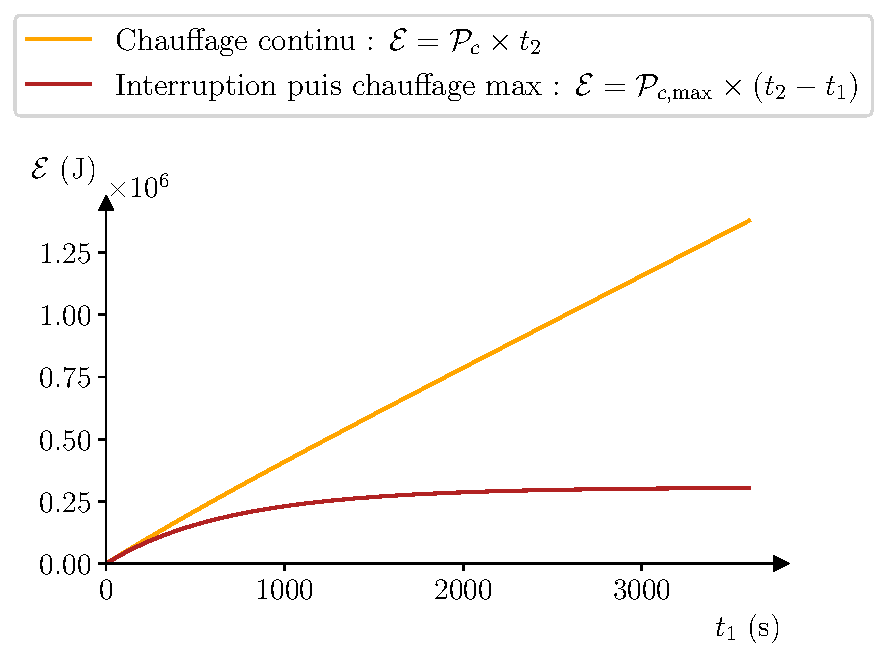
\includegraphics[width=\linewidth]{E7_solve_t1_egal}
		\end{center}
	\end{minipage}
	\hfill
	\begin{minipage}[c]{.50\linewidth}
		On observe que la méthode de \textbf{maintenir le chauffage} est
		\textbf{toujours pire} que le fait de l'arrêter, même si c'est pour le
		relancer avec une plus grande puissance. Il n'y a que pout $t_1 \to 0$ que
		les deux méthodes sont semblables. Ainsi, \textbf{il vaut toujours mieux
			couper le chauffage en sortant}~!
	\end{minipage}
}%

\end{document}
